\chapter{基礎概念}
\label{chap:concept}

\section{アドホックネットワーク}
アドホックネットワークとは,アクセスポイントを必要としない無線で接続できる端末のみで構成されたネットワークである.
直接電波が届き通信可能である場合には,始点ノードから終点ノードへ1ホップでパケット伝達が行われる.電波が直接届かない場合にはノードを経由(マルチホップ)することで終点ノードまでパケットを伝達する.
端末の中継機能を利用してネットワークを構成しているので,アドホックネットワークには基地局インフラが不要である.

\section{AllJoyn}
AllJoynはQualcommが開発したオープンソースプロジェクトである.デバイス間通信を実現し,製品やアプリケーション間の相互運用を可能にするデバイス通信フレームワークを提供している.
Android,iOS,OS X,Linux,Windows7など様々なOSに対応し,Java,C++,C,JavaScriptなどの言語で使用できる.
AllJoynは近傍デバイスの探索やP2Pネットワークへの接続,セキュリティなどの要素を提供しており,機器やOSに依存せず開発することができる.


AllJoynネットワークはAllJoynアプリケーションとAllJoynルーターから成る.
AllJoynアプリケーションはAllJoynルーターを通じて他のAllJoynアプリケーションと通信を行う.
AllJoynアプリケーションは以下の要素から成る.

\begin{itemize}
\item AllJoyn App Cods
\item AllJoyn Service Frameworks Libraries
\item AllJoyn Core Library
\end{itemize}

\begin{figure}
\centering
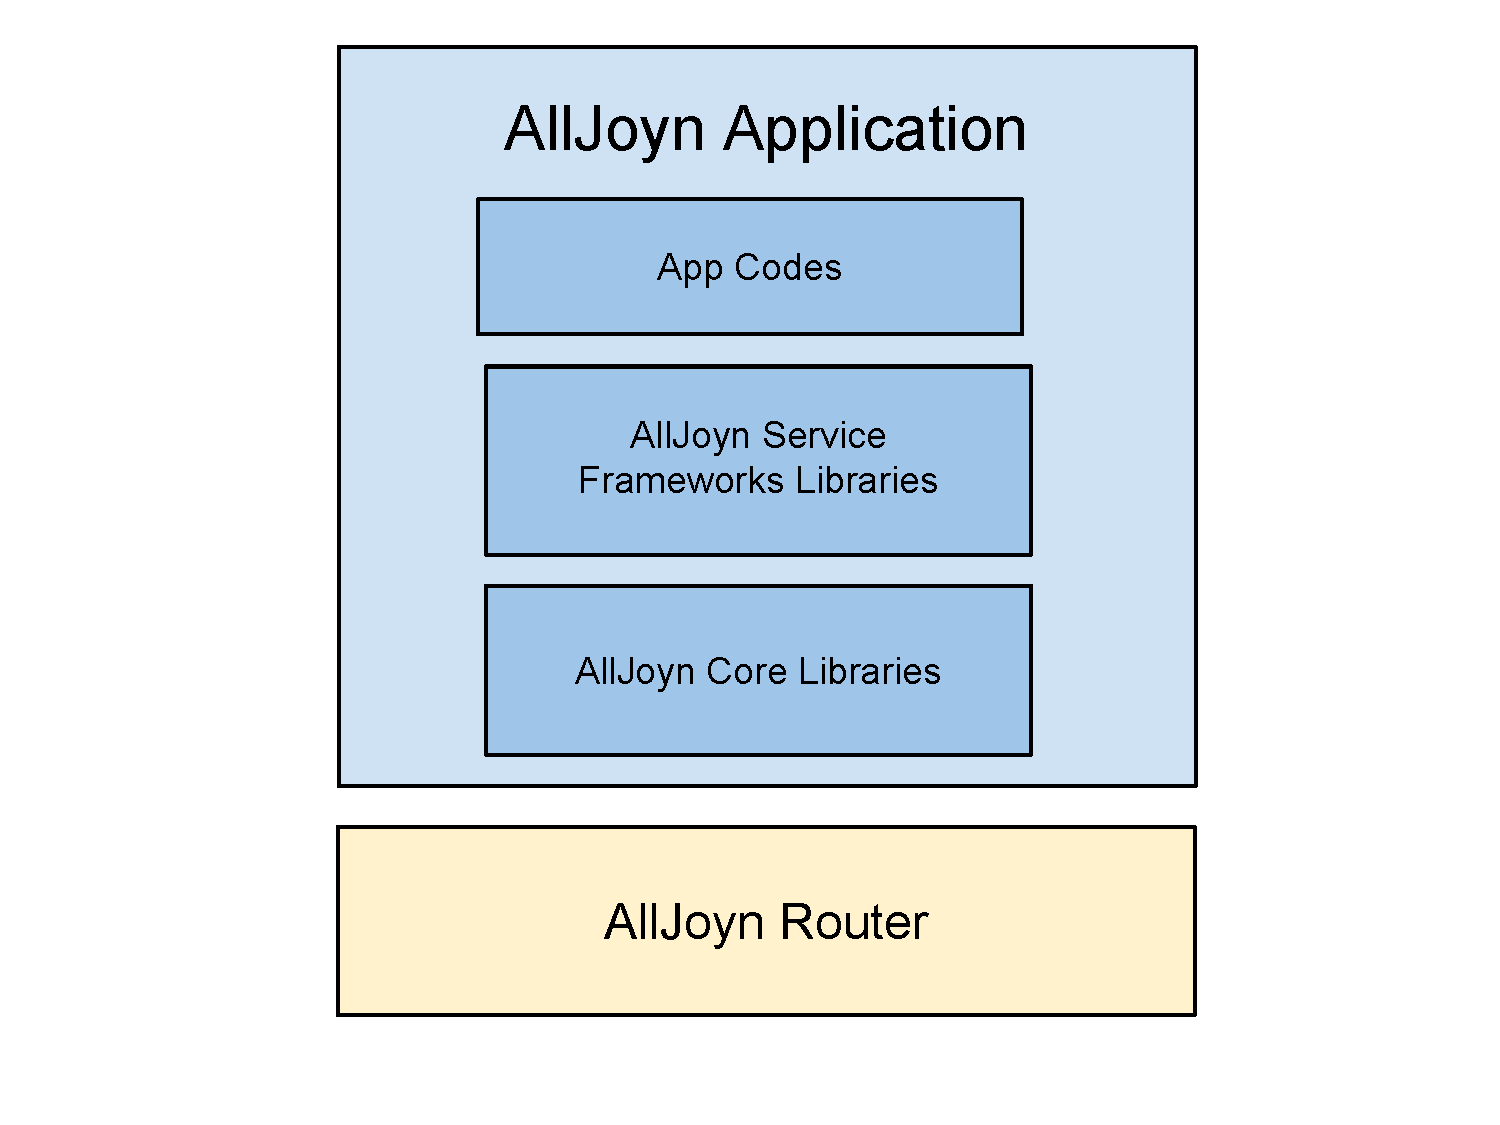
\includegraphics[width=15cm]{fig/AllJoyn.pdf}
\end{figure}

\subsection{AllJoyn Core Library}
AllJoyn Core LibraryはAllJoynネットワークと通信するための最低限のAPIを提供する.
提供するAPIは以下の通りである.

\begin{itemize}
\item Advertisements
\item Discovery
\item Session creation
\item Interface definition of methods, properties, and signals
\item Object creation and handling
\end{itemize}

\subsection{AllJoyn Service Framework Libraries}
AllJoyn Service Framework Librariesは,onboarding,notificatino,control panelなどのサービスを備えている.
Base Servicesとして以下の機能がある.

\begin{itemize}
\item Base Services
\begin{itemize}
\item Onbording \\ 
Wi-Fiネットワークへの接続をサポート
\item Configuration \\
デバイスの構成
\item Notificatinos \\
デバイスからの通知
\item Control Panel \\
UI widgetとリモートデバイスとの通信
\end{itemize}
\end{itemize}

AllJoyn Service Framework Librariesを使うことで,アプリケーションやデバイスは互いにこれらのサービスを運用することができる.


\subsection{AllJoyn App Code}
AllJoyn App CodeはAllJoynアプリケーションのロジックである.
高レベルの機能を提供するAllJoyn Service Frameworksか直接AllJoyn Core APIにアクセスできるAllJoyn Core Libraryのどちらかを用いてプログラミングされる.

\subsection{AllJoyn Router}


\section{iBeacon}
iBeacon\cite{iBeacon}は,2013年にAppleが発表したBluetooth Low Energy(BLE)を利用した技術であり,発信機から発せられるビーコンを受信し,発信機の位置を特定・確認できる.
Bluetooth Low Energy(BLE)は名前の通り低電力仕様であり,発信機はボタン電池1つで1年以上稼働することができるといわれている.
iOS7以降のデバイス(iPhone,iPad,およびiPod touch)やAndroid4.3以降のデバイスなどで受信することができる.
iBeaconでは領域の出入りをチェックするリージョン監視やビーコンの情報を受信するレーシングを用いて位置や近接具合などを検知する.
ビーコンを受信したときに得られる情報には以下の6つがある.

\begin{center}
\begin{table}[htb]
\begin{tabular}{|l|l|}  \hline
proximityUUID & 識別子 \\ \hline
major & 識別子 \\  \hline
minor & 識別子 \\ \hline
proximity & ビーコンとの距離 \\ \hline
accuracy & 距離の精度 \\ \hline
rssi & 受信強度 \\ \hline
\end{tabular}
\end{table}
\end{center}

また,proximityは正確な距離を表すものではなく,以下の大まかな4つの値で得ることができる.

\begin{center}
\begin{table}[htb]
\begin{tabular}{|l|l|} \hline
Unknown & 検出不可 \\ \hline
Immediate & 至近距離 \\ \hline
Near & 近距離 \\ \hline
Far & 遠距離 \\ \hline
\end{tabular}
\end{table}
\end{center}
